\title{Systematic Review}
\author{
	Jomar Alcantara \\
	Department of Computer Science\\
	School of Engineering and Applied Sciences\\
	Aston University
	\and
	Peter Sawyer \\
	Department of Computer Science\\
	School of Engineering and Applied Sciences\\
	Aston University
	\and
	George Vogiatzis\\
	Department of Computer Science\\
	School of Engineering and Applied Sciences\\
	Aston University}
	
\date{\today}

\documentclass[12pt]{article}

\usepackage[utf8]{inputenc}
\usepackage{tikz}
\usetikzlibrary{shapes.geometric, arrows}

\tikzstyle{startstop} = [rectangle, rounded corners, minimum width=3cm, minimum height=1cm,text centered, draw=black, fill=red!30]
\tikzstyle{io} = [trapezium, trapezium left angle=70, trapezium right angle=110, minimum width=3cm, minimum height=1cm, text centered, draw=black, fill=blue!30]
\tikzstyle{process} = [rectangle, minimum width=3cm, minimum height=1cm, text centered, text width=3cm, draw=black, fill=orange!30]
\tikzstyle{decision} = [diamond, minimum width=3cm, minimum height=1cm, text centered, draw=black, fill=green!30]
\tikzstyle{arrow} = [thick,->,>=stealth]

\begin{document}
\maketitle

\begin{abstract}
This is the paper's abstract \ldots
\end{abstract}

\section{Introduction}
Dementia has been identified as one of those fast growing difficulties facing the world. A recent report suggests that in 2015 there were 46 million people with a diagnosis of dementia and that number is expected to hit 131.5 million by 2050 \cite{Prince2015}. The report also states that the worldwide cost of dementia in 2018 is estimated to be in the region of one trillion US dollars.
\par
In 2009, the Department of Health designed it's National Dementia strategy and as part of this made early diagnosis and support one of it's key priorities \cite{England2009}. A lot of work has gone into trying to find ways of improving the early diagnosis of Alzheimer's Disease (AD) and Mild Cognitive Impairment (MCI) with research focused on two areas - identifying biological markers and analyzing the cognitive decline of those who are suspected to have the disease \cite{Taler2008}. As described above, the numbers of those suffering from AD and MCI are going to increase as the population ages \cite{Prince2015} and thus it is important that we utilize technology wherever possible to aid clinicians in the detection of MCI and AD. At the present time diagnosis is typically conducted at memory clinics by trained clinicians \cite{Boschi2017}. I theorize that we may be able to enable an earlier diagnosis of those with MCI and AD using samples of spontaneous speech, natural language processing (NLP) and machine learning (ML).
\par
There is a large body of research that looks at the decline in language in those with MCI and AD \cite{Taler2008, Boschi2017}. However there is conflicting evidence in these studies about which declining language factors are associated of MCI and AD \cite{Taler2008, Boschi2017}. Research therefore should look at these features in more detail and a clarification of this currently disorganised picture should go some way to helping researchers further understand the disease and it's progression. Another area of focus for research of this nature is the process of collecting appropriate language samples. Whilst collecting samples of language is comparatively unintrusive, researchers recognise that these samples require a rich sample of language that potentially cannot be generated by tasks such as the picture description task. Therefore, it would be useful to explore whether spontaneous discourse such a semi-structured interview, has the ability to put pressure on both the cognitive and linguistic systems in the same way as traditional cognitive tests such that it might be able to distinguish between healthy controls, those with MCI and those with AD. There is some evidence to support this. Berisha et al \cite{Berisha2015}, has shown through a longitudinal language analysis of spontaneous speech that there are marked differences in this process between those who would go on to have a diagnosis of AD and a healthy control. 
\par
The potential impact of this research in this area is immense. Research has shown that early diagnosis of people with AD or MCI improves sufferers quality of life and can, in some cases, slow the progress of the disease. Early diagnosis can increase the number of research opportunities for understanding the early stages of dementia and how the disease progresses so that more research can be conducted which may, in the future, lead to new treatments and other interventions.

The aim of my research is to find less burdensome ways of detecting dementia without the use of invasive procedures (taking bloods, or using medical equipment such as MRI's and EEG's) and without resorting to to time-consuming and expensive psychological tests. There is a lot of research into the analysis of language as a bio-marker for MCI and Early Dementia. Given that sampling a person's language is relatively effortless, my research looks at whether we can find bio-markers of MCI and Early Dementia in natural language.\newline
Concerns: Language and Memory are quite naturally intertwined and it would be difficult to test one without some reliance on the other. I'm not going to control for memory problems as a potential confound, but does this weaken the research? How do I defend this? \newline
\par 
Introduction to the problem of dementia in the context of the wider world including quality of life and financial implications. Exploration of dementia as a syndrome rather than a disease, and a look at the different variants of dementia. A look at the rationale behind research into the early diagnosis of dementia as well as a brief look at what has been done in the area (wide context, so pharmacological and psychological). \newline

The question to be addressed in this systematic review is how has the field of machine learning and natural language processing addresses language deterioration in the diagnosis of Mild Cognitive Impairment and Early Alzheimer's Disease.

The remainder of this article is organized as follows. Section~\ref{methodology} gives an account of the process of this Systematic Review. Our new and exciting results are described in Section~\ref{results}. We discuss the results and implications in Section~\ref{discussion}. Finally, Section~\ref{conclusions} gives the conclusions.

\section{Methodology}\label{methodology}

A systematic literature review (SLR) describes a process which aims to identify, evaluate and interpret the research and literature in a given area. They are designed to provide a complete and exhaustive summary of the current evidence relevant to an identified research question. SLR's conduct a thorough search of all literature following a pre-defined protocol that specifies focused research questions, identifies criteria for the selection of studies and assessment of their quality, and forms to execute the data extraction and synthesis of results. 
\par 
Common motivations for conducting a SLR are: 
\begin{enumerate}
	\item to summary all the evidence about a topic.
	\item find gaps in the research. 
	\item to provide a ground for a fundament to new research.
	\item and to examine how the current research supports a hypothesis. 
\end{enumerate}

Performing a SLR comprises the following steps: 
\begin{enumerate}
	\item (i) identify the need for performing the SLR.
	\item (ii) formulate research questions.
	\item (iii) execute a comprehensive search and selection of primary studies.
	\item (iv) assess the quality and extract data from the studies.
	\item (v) interpret the results.
	\item (vi) report the SLR.
\end{enumerate}

The main research question this SLR aims to address is: “How has the field of machine learning and natural language processing addresses language deterioration in the diagnosis of Mild Cognitive Impairment and Early Alzheimer's Disease?”. This main question was decomposed further into five research questions:
\begin{enumerate}
	\item RQ1: Which ML and MS techniques are being used in the dementia and comorbidities research?
	\item RQ2: What data characteristics (variables, determinants and indicators) are being considered when applying the ML or/and MS techniques (physiological, demographic/social, genetics, lifestyle etc)?
	\item RQ3: What are the goals of the studies that employ ML or MS techniques for prognosis of dementia and comorbidities?
	\item RQ4: How is data censoring being handled in the studies?
	\item RQ5: Do the studies focus on individuals or populations?
\end{enumerate}

The present paper builds upon these questions and additionally presents the results of the other two additional research questions. Further, the key terms related to comorbidities were included in the search string to ensure that relevant studies about ML or MS for the prognosis of a disease, where dementia is considered a comorbidity to that disease would also be retrieved from the database searches, even when the term dementia was not mentioned in the paper’s title or abstract.

\subsection{Search strategy}
To address the research questions, a search string was defined using the PICO approach, which decomposes the main question into four parts: population, intervention, comparison and outcome. The comparison component was discarded because the SLR was mainly concerned with a characterization. For each of the remaining components, keywords were derived and their rationale can be represented as follows:
\begin{enumerate}
	\item Population: Studies that present research on dementia and comorbidities. Dementia’s keywords were selected from the “Systematized Nomenclature of Medicine–Clinical Terms” and selected by A4. Comorbidities’ keywords were extracted from the Marengoni et al. SLR in this topic.
	\item Intervention: ML or MS techniques. The ML keywords were selected from the branch “Machine Learning Approaches” of the “2012 ACM Computing Classification System”. The MS keywords were selected by A2.
	\item Outcome: Prognosis on dementia and comorbidies. The prognosis keywords were provided
by A4.
\end{enumerate}

The automated searches were performed in the Pubmed, Web of Science and Scopus databases. Table 1 shows the search string used for the Pubmed automated search, but note that this search string was adapted to each of the other databases’ search context.

\begin{table}
	\begin{tabular}{ p{12cm} }
	\hline
	(dementia OR MCI OR Mild Cognitive Impairment OR Alzheimer's OR Mild Neurocognitive Disorder OR AD) AND TOPIC: (machine learning OR Data Mining OR Decision Support System OR NLP OR Natural 			Language Processing) AND TOPIC: (prognosis OR prognostic estimate OR predictor OR prediction OR model OR patterns OR diagnosis OR diagnostic OR forecasting OR projection OR Deep Language Model 		OR Deep Neural Network) AND TOPIC: (classification OR regression OR kernel OR support vector machines OR Gaussian Process OR Bayesian Network OR Factor Analysis OR Deep Learning OR Neural 			Networks OR Maximum Likelihood OR Principal Component Analysis OR Markov OR Linear Model OR Mixture Model OR Perceptron Algorithm OR Logical Learning OR relational learning OR Supervised 				Learning OR Unsupervised Learning OR clustering OR Decision Tree) AND TOPIC: (Language OR Cognitive OR Speech OR Conversation OR Connected Speech OR Picture Description OR Discourse Analysis OR 		Verbal Fluency)  \\ \hline
	Searched - 4th April 2019 - Generated 1257 Articles \\
	\hline
	\end{tabular}
	\caption[Table caption text]{Search Terms for Web of Science database}
	\label{table:name}
\end{table}

\begin{table}
	\begin{tabular}{ p{12cm} }
	\hline
	(dementia OR MCI OR Mild Cognitive Impairment OR Alzheimer's OR Mild Neurocognitive Disorder OR AD) AND TOPIC: (machine learning OR Data Mining OR Decision Support System OR NLP OR Natural 			Language Processing) AND TOPIC: (prognosis OR prognostic estimate OR predictor OR prediction OR model OR patterns OR diagnosis OR diagnostic OR forecasting OR projection OR Deep Language Model 		OR Deep Neural Network) AND TOPIC: (classification OR regression OR kernel OR support vector machines OR Gaussian Process OR Bayesian Network OR Factor Analysis OR Deep Learning OR Neural 			Networks OR Maximum Likelihood OR Principal Component Analysis OR Markov OR Linear Model OR Mixture Model OR Perceptron Algorithm OR Logical Learning OR relational learning OR Supervised 				Learning OR Unsupervised Learning OR clustering OR Decision Tree) AND TOPIC: (Language OR Cognitive OR Speech OR Conversation OR Connected Speech OR Picture Description OR Discourse Analysis OR 		Verbal Fluency)  \\ \hline
	Searched - 4th April 2019 - Generated 1257 Articles \\
	\hline
	\end{tabular}
	\caption[Table caption text]{Search Terms for Scopus database}
	\label{table:name}
\end{table}

\begin{table}
	\begin{tabular}{ p{12cm} }
	\hline
	(dementia OR MCI OR Mild Cognitive Impairment OR Alzheimer's OR Mild Neurocognitive Disorder OR AD) AND TOPIC: (machine learning OR Data Mining OR Decision Support System OR NLP OR Natural 			Language Processing) AND TOPIC: (prognosis OR prognostic estimate OR predictor OR prediction OR model OR patterns OR diagnosis OR diagnostic OR forecasting OR projection OR Deep Language Model 		OR Deep Neural Network) AND TOPIC: (classification OR regression OR kernel OR support vector machines OR Gaussian Process OR Bayesian Network OR Factor Analysis OR Deep Learning OR Neural 			Networks OR Maximum Likelihood OR Principal Component Analysis OR Markov OR Linear Model OR Mixture Model OR Perceptron Algorithm OR Logical Learning OR relational learning OR Supervised 				Learning OR Unsupervised Learning OR clustering OR Decision Tree) AND TOPIC: (Language OR Cognitive OR Speech OR Conversation OR Connected Speech OR Picture Description OR Discourse Analysis OR 		Verbal Fluency)  \\ \hline
	Searched - 4th April 2019 - Generated 1257 Articles \\
	\hline
	\end{tabular}
	\caption[Table caption text]{Search Terms for ProQuest database}
	\label{table:name}
\end{table}

\begin{table}
	\begin{tabular}{ p{12cm} }
	\hline
	(dementia OR MCI OR Mild Cognitive Impairment OR Alzheimer's OR Mild Neurocognitive Disorder OR AD) AND TOPIC: (machine learning OR Data Mining OR Decision Support System OR NLP OR Natural 			Language Processing) AND TOPIC: (prognosis OR prognostic estimate OR predictor OR prediction OR model OR patterns OR diagnosis OR diagnostic OR forecasting OR projection OR Deep Language Model 		OR Deep Neural Network) AND TOPIC: (classification OR regression OR kernel OR support vector machines OR Gaussian Process OR Bayesian Network OR Factor Analysis OR Deep Learning OR Neural 			Networks OR Maximum Likelihood OR Principal Component Analysis OR Markov OR Linear Model OR Mixture Model OR Perceptron Algorithm OR Logical Learning OR relational learning OR Supervised 				Learning OR Unsupervised Learning OR clustering OR Decision Tree) AND TOPIC: (Language OR Cognitive OR Speech OR Conversation OR Connected Speech OR Picture Description OR Discourse Analysis OR 		Verbal Fluency)  \\ \hline
	Searched - 4th April 2019 - Generated 1257 Articles \\
	\hline
	\end{tabular}
	\caption[Table caption text]{Search Terms for IEEE Xplore database}
	\label{table:name}
\end{table}

\subsection{Study selection}
The first step of the study selection was the execution of an evaluation round with 100 random papers from the 593 results returned from the automated searches. These had their title and abstracts assessed by A1, A2 and A3, according to inclusion and exclusion criteria defined previously in the protocol (see Table 2). This step was mainly concerned in maintaining the consistency of the selection between the participants throughout the SLR. The remaining 493 results had their title and abstracts assessed by A1 and A2, according to the inclusion and exclusion criteria. After the evaluations, 37 papers were selected. Then a one-iteration backward snowballing was carried out looking for possible additional studies. The 1199 new identified studies were assessed analogously as the previous ones, resulting in 41 new selected papers. Throughout the whole selection process, A3 and A4 acted in conflict resolution in the case where A1 and A2 couldn’t reach an agreement.
\par 
In total, 78 papers were selected to be fully read and assessed regarding its eligibility. The ones that successfully passed the established criteria previously defined in the protocol, had their relevant data extracted. In order to minimize the chance of selecting studies with bias evidence, a quality assessment questionnaire was used. This questionnaire was adapted from Kitchenham’s guidelines and can be found in the SLR protocol. If the grading attributed to a paper fell below 8 points (out of a total of 12), it would be rejected for quality reasons. The 8-point threshold was
decided in the research group discussions involving all the authors. In this phase, a paper could also be rejected due to inclusion and exclusion criteria because the selection process adopted an inclusive approach. This means that during the reading of the titles and abstracts, in the case where the information provided was incomplete or too general it was selected to be fully read in the posterior phase. A common example is the case when the data analysis technique specified in the abstract was merely “classification”, so it was not possible to know if any machine learning occurred.
\par
As in the study selection, a quality assessment evaluation round was performed beforehand to ensure consistency in the evaluations. A1, A2 and A5 participated in this task. In total, 37 studies composed the final set of included primary studies and had their relevant data extracted, 7 papers were rejected due quality reasons, and 34 papers were rejected due to failing the inclusion and exclusion criteria. One reason for the high number of the latter was the decision to exclude the papers that used solely statistical methods as data analysis tech- niques to build the prognostic models. The selected studies were also assessed for the risk of cumulative evidence bias. This was done by checking, in the case of the same research group with different studies in the final set of included primary studies, if it was justified having both studies (i.e different samples).

\subsection{Data collection}
For the data collection, a base extraction form was defined in the protocol, but later in the study it was evolved based on the research group discussions. Table 3 lists and defines the collected variables.

\begin{table}
	\begin{tabular}{ p{6cm} | p{6cm} }
	\hline
	Inclusion Criteria & Exclusion Criteria \\ \hline
	Be a primary study in English; AND address research on dementia and comorbidities; AND address at least one ML or MS technique; AND address a prognosis related to dementia and comorbidities. &
	Be a secondary or tertiary study; OR be written in another language other than English; OR do not address a research on dementia and comorbidities; OR do not address at least one ML or MS technique; OR do not address a prognosis related to dementia and comorbidities. \\
	\hline 
	\end{tabular}
	\caption[Table caption text]{Inclusion and Exclusion Criteria}
	\label{table:name}
\end{table}

\begin{table}
	\begin{tabular}{ p{6cm} | p{6cm} }
	\hline
	Variable & Definition \\ \hline
	Conditions Studied & For which dementia disorder is the study deriving a prognosis. \\ \hline
	Database used in the study & Name and origin of the data source used to derive the prognosis of the studied dementia. \\ \hline
	Dataset Categories & Classes in which the data units were divided into. \\ \hline
	Handling of Censored Data & Description of the way in which censored data was handled. \\ \hline
	Follow-up period & Period of time, which the data units were followed. \\ \hline
	Data Analysis Techniques & ML or MS techniques that were used to build the prognostic models. \\ \hline 
	Model Variables & The variables used in building the prognostic models. \\ \hline
	Aim of the Study & The goal of the built prognostic models. \\ \hline 
	Focus of the Study & If the built prognostic models aim its predictions on an individual or population level. \\
	\hline 
	\end{tabular}
	
\end{table}

In addition to these variables other basic data about the studies was collected, these were: title, authors, journal/source, year and type of publication. No summary measures were used. Summary tables were used for the synthesis of results and no additional analyses were carried out

\section{Results}\label{results}
In this section we describe the results.

\begin{figure}


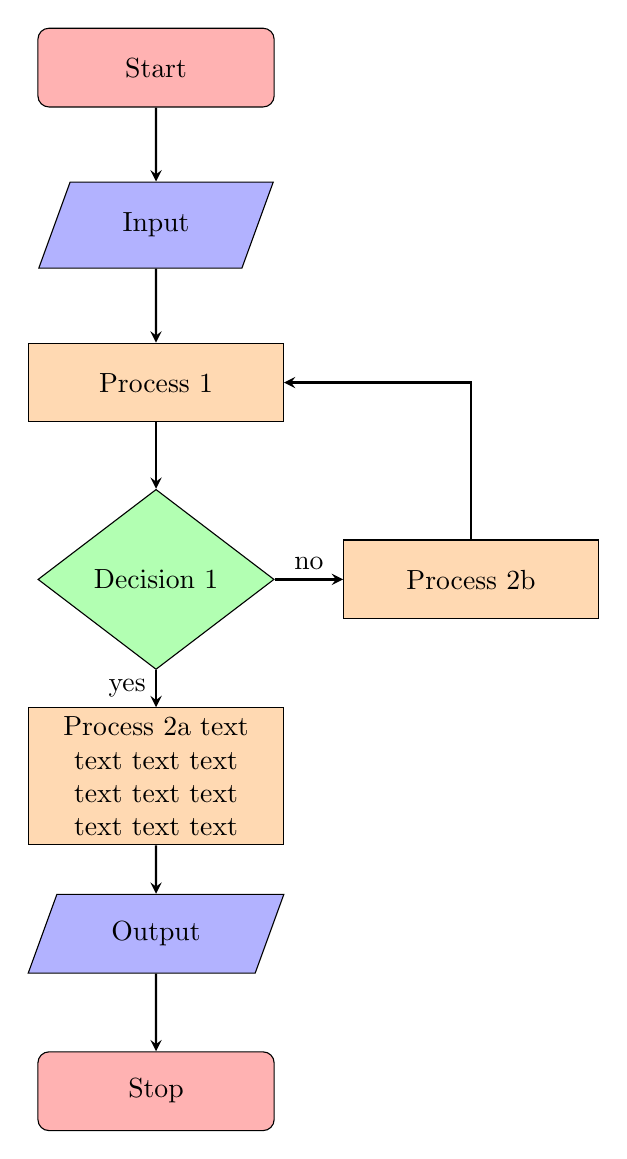
\begin{tikzpicture}[node distance=2cm]

\node (start) [startstop] {Start};
\node (in1) [io, below of=start] {Input};
\node (pro1) [process, below of=in1] {Process 1};
\node (dec1) [decision, below of=pro1, yshift=-0.5cm] {Decision 1};
\node (pro2a) [process, below of=dec1, yshift=-0.5cm] {Process 2a text text text text text text text text text text};
\node (pro2b) [process, right of=dec1, xshift=2cm] {Process 2b};
\node (out1) [io, below of=pro2a] {Output};
\node (stop) [startstop, below of=out1] {Stop};

\draw [arrow] (start) -- (in1);
\draw [arrow] (in1) -- (pro1);
\draw [arrow] (pro1) -- (dec1);
\draw [arrow] (dec1) -- node[anchor=east] {yes} (pro2a);
\draw [arrow] (dec1) -- node[anchor=south] {no} (pro2b);
\draw [arrow] (pro2b) |- (pro1);
\draw [arrow] (pro2a) -- (out1);
\draw [arrow] (out1) -- (stop);
\end{tikzpicture}
\caption[Figure caption text]{PRISMA flow chart.}
\label{figure:name}
\end{figure}
\subsection{Language Analysis of Speakers with Dementia of the Alzheimer's Type - Guinn and Habash (2012)}

\subsection{Features and Machine Learning Classification of Connected Speech Samples from patients with Autopsy Proven Alzheimer's Disease with and without additional Vascular Pathology - Rentoumi, Raoufian, Ahmed, de Jager, Garrard (2014)}

\subsection{Learning Predictive Linguistic Features for Alzheimer's Disease and related Dementias using Verbal Utterances - Orimaye, Wong and Golden (2014)}

\subsection{Learning Lingustic Biomarkers for Predicting Mild Cognitive Impairment using Compound Skip-grams - Orimaye, Wong, Wong and Tai (2015)}

\subsection{Diagnosing People with Dementia using Automatic Conversation Analysis - Mirheidari, Reuber, Blackburn, Walker (2016)}

\subsection{Formulaic Language in People with Probably Alzheimer's Disease: A Frequency-Based Approach - Zimmerer, Wibrow and Varley (2016)}

\subsection{Linguistic Features Identify Alzheimer's Disease in Narrative Speech - Fraser, Melzer and Rudzicz (2016}

\subsection{Declines in Connected Language Are Associated with Very Early Mild Cognitive Impairment: Results from the Wisconsin Registry for Alzheimer's Prevention - Mueller, Koscik, Hermann, Johnson and Turkstra (2018)}

\subsection{Deep language space neural network for classifying mild cognitive impairment and Alzheimer-type dementia - Orimaye, Wong and Wong (2018)}
In this paper, Orimaye et al use deep-deep neural networks language models (D2NNLM) to learn linguistic changes that distinguish the language of patients with MCI and AD-type dementia from the healthy controls using higher order n-grams. An ordinary DNNLM uses lower order n-gram N-dimensional sparse vectors as descrete feature representations to train the neural network with multiple hidden layers.

\subsubsection{Deep Neural Network Language Models}

\section{Discussion}\label{discussion}

\section{Conclusions}\label{conclusions}
We worked hard, and achieved very little.



\bibliographystyle{abbrv}
\bibliography{main}

\end{document}
